\documentclass[]{article}
\usepackage{lmodern}
\usepackage{amssymb,amsmath}
\usepackage{ifxetex,ifluatex}
\usepackage{fixltx2e} % provides \textsubscript
\ifnum 0\ifxetex 1\fi\ifluatex 1\fi=0 % if pdftex
  \usepackage[T1]{fontenc}
  \usepackage[utf8]{inputenc}
\else % if luatex or xelatex
  \ifxetex
    \usepackage{mathspec}
    \usepackage{xltxtra,xunicode}
  \else
    \usepackage{fontspec}
  \fi
  \defaultfontfeatures{Mapping=tex-text,Scale=MatchLowercase}
  \newcommand{\euro}{€}
\fi
% use upquote if available, for straight quotes in verbatim environments
\IfFileExists{upquote.sty}{\usepackage{upquote}}{}
% use microtype if available
\IfFileExists{microtype.sty}{%
\usepackage{microtype}
\UseMicrotypeSet[protrusion]{basicmath} % disable protrusion for tt fonts
}{}
\usepackage[margin=1in]{geometry}
\usepackage{color}
\usepackage{fancyvrb}
\newcommand{\VerbBar}{|}
\newcommand{\VERB}{\Verb[commandchars=\\\{\}]}
\DefineVerbatimEnvironment{Highlighting}{Verbatim}{commandchars=\\\{\}}
% Add ',fontsize=\small' for more characters per line
\usepackage{framed}
\definecolor{shadecolor}{RGB}{248,248,248}
\newenvironment{Shaded}{\begin{snugshade}}{\end{snugshade}}
\newcommand{\KeywordTok}[1]{\textcolor[rgb]{0.13,0.29,0.53}{\textbf{{#1}}}}
\newcommand{\DataTypeTok}[1]{\textcolor[rgb]{0.13,0.29,0.53}{{#1}}}
\newcommand{\DecValTok}[1]{\textcolor[rgb]{0.00,0.00,0.81}{{#1}}}
\newcommand{\BaseNTok}[1]{\textcolor[rgb]{0.00,0.00,0.81}{{#1}}}
\newcommand{\FloatTok}[1]{\textcolor[rgb]{0.00,0.00,0.81}{{#1}}}
\newcommand{\CharTok}[1]{\textcolor[rgb]{0.31,0.60,0.02}{{#1}}}
\newcommand{\StringTok}[1]{\textcolor[rgb]{0.31,0.60,0.02}{{#1}}}
\newcommand{\CommentTok}[1]{\textcolor[rgb]{0.56,0.35,0.01}{\textit{{#1}}}}
\newcommand{\OtherTok}[1]{\textcolor[rgb]{0.56,0.35,0.01}{{#1}}}
\newcommand{\AlertTok}[1]{\textcolor[rgb]{0.94,0.16,0.16}{{#1}}}
\newcommand{\FunctionTok}[1]{\textcolor[rgb]{0.00,0.00,0.00}{{#1}}}
\newcommand{\RegionMarkerTok}[1]{{#1}}
\newcommand{\ErrorTok}[1]{\textbf{{#1}}}
\newcommand{\NormalTok}[1]{{#1}}
\usepackage{graphicx}
\makeatletter
\def\maxwidth{\ifdim\Gin@nat@width>\linewidth\linewidth\else\Gin@nat@width\fi}
\def\maxheight{\ifdim\Gin@nat@height>\textheight\textheight\else\Gin@nat@height\fi}
\makeatother
% Scale images if necessary, so that they will not overflow the page
% margins by default, and it is still possible to overwrite the defaults
% using explicit options in \includegraphics[width, height, ...]{}
\setkeys{Gin}{width=\maxwidth,height=\maxheight,keepaspectratio}
\ifxetex
  \usepackage[setpagesize=false, % page size defined by xetex
              unicode=false, % unicode breaks when used with xetex
              xetex]{hyperref}
\else
  \usepackage[unicode=true]{hyperref}
\fi
\hypersetup{breaklinks=true,
            bookmarks=true,
            pdfauthor={Petr Keil, pkeil@seznam.cz},
            pdftitle={Template for writing scientific papers in R markdown},
            colorlinks=true,
            citecolor=blue,
            urlcolor=blue,
            linkcolor=magenta,
            pdfborder={0 0 0}}
\urlstyle{same}  % don't use monospace font for urls
\setlength{\parindent}{0pt}
\setlength{\parskip}{6pt plus 2pt minus 1pt}
\setlength{\emergencystretch}{3em}  % prevent overfull lines
\setcounter{secnumdepth}{5}

%%% Use protect on footnotes to avoid problems with footnotes in titles
\let\rmarkdownfootnote\footnote%
\def\footnote{\protect\rmarkdownfootnote}

%%% Change title format to be more compact
\usepackage{titling}
\setlength{\droptitle}{-2em}
  \title{Template for writing scientific papers in R markdown}
  \pretitle{\vspace{\droptitle}\centering\huge}
  \posttitle{\par}
  \author{Petr Keil, \href{mailto:pkeil@seznam.cz}{\nolinkurl{pkeil@seznam.cz}}}
  \preauthor{\centering\large\emph}
  \postauthor{\par}
  \predate{\centering\large\emph}
  \postdate{\par}
  \date{11/1/2015}




\begin{document}

\maketitle


\section{Resumen}\label{resumen}

En este trabajo se presenta el paquete WindResource para el software
estadístico libre R. Se trata de la primera versión de del software
actualmente en desarrollo en el marco del proyecto UTN 1894.\\Este
paquete incluye funciones para el estudio del recurso eólico. Mediante
estas funciones es posible realizar un análisis descriptivo exhaustivo
de las características del viento. Estos análisis son imprescindibles a
la hora de evaluar el potencial de un determinado sitio donde se
pretenda instalar aerogeneradores con fines energéticos.\\El software
permite análisis de frecuencias de velocidad y dirección, ajustar
distribuciones, y obtener proyecciones de la energía anual
generada.\\Para simplificar la operación del paquete, se ha integrado al
mismo una interfaz web utilizando el paquete Shiny.\\Se describen en
este trabajo las principales características funcionales de esta primera
versión del software.

\section{1. Introduccion}\label{introduccion}

La medición del recurso eólico es uno de los pilares fundamentales para
la caracterización de un sitio en donde se pretenda instalar una planta
de generación de energía eléctrica a través de turbinas de viento. La
correcta estimación del potencial eólico de una región es de vital
importancia a la hora de evaluar proyectos de inversión y sobre todo
solicitar financiamiento para los mismos.\\Al ser la velocidad de viento
una variable aleatoria, la correcta identificación de la distribución y
sus parámetros es fundamental en la determinación del potencial eólico.
Argentina es reconocida internacionalmente como uno de los países con
mayor potencial para el desarrollo eólico. Dominada en su matriz
energética eléctrica por la generación convencional fósil, cuenta con
posibilidades inigualables en cuanto a recursos eólicos. Posee
velocidades medias de viento en la mayor parte de su territorio, medidas
a 50 metros de altura, que superan los 6 metros por
segundo.\\Actualmente el país cuenta aproximadamente con una potencia
instalada a través de energía eólica que representa aproximadamente el
0,4\% de la capacidad instalada total.\\De acuerdo la Ley 26.190 de
energías renovables, para el 2016 se deberá llegar al 8\% de la matriz
eléctrica con energía renovable. Para poder cumplir con este
requerimiento, en el año 2010 se licitaron a través del GENREN alrededor
de 900 MW para generación de energías renovables. De este total, 754 MW
tendrán como fuente la energía eólica. Teniendo en cuenta que hasta el
momento de la licitación, la Argentina solo contaba con 30MW de potencia
instalada que utilizaban este tipo de energía, podemos tomar conciencia
de la magnitud en el cambio propuesto.

\section{2. Preparación}\label{preparacion}

\subsection{2.1. Preparación R}\label{preparacion-r}

La primera versión del paquete WindResorce se encuentra disponible en el
CRAN de R. Con lo cual solo bastará con instalar el paquete utilizando
el comando:

\begin{Shaded}
\begin{Highlighting}[]
\KeywordTok{install.packages}\NormalTok{(}\StringTok{"WindResource"}\NormalTok{)}
\end{Highlighting}
\end{Shaded}

y luego cargar la librería en memoria:

\begin{Shaded}
\begin{Highlighting}[]
\KeywordTok{library}\NormalTok{(WindResource)}
\end{Highlighting}
\end{Shaded}

El código fuente de la versión en desarrollo se encuentra disponible en
GitHub: \url{https://github.com/mbonoli/WindResource}. También es
posible instalar en R los comnados correspondientes de la siguiente
utilizando el comando install\_github disponible en el paquete devtool:

\begin{Shaded}
\begin{Highlighting}[]
\KeywordTok{library}\NormalTok{(devtools)}
\KeywordTok{install_github}\NormalTok{(}\StringTok{"mbonoli/WindResource"}\NormalTok{)}
\end{Highlighting}
\end{Shaded}

\subsection{2.2. Preparación de los
datos}\label{preparacion-de-los-datos}

Para ejemplificar, utilizaremos los datos provenientes de una torre de
medición situada en XXXX. La información acerca del origen de los datos
en encuentra disponible en al siguiente dirección:
\href{http://www.umass.edu/windenergy/publications/resource/Mt_Tom_Holyoke}{\url{http://www.umass.edu/windenergy/publications/resource/Mt_Tom_Holyoke}}.
En particular trabajaremos con el set de datos de del período 1999-2002,
almacenado en el archivo
\href{http://www.umass.edu/windenergy/publications/resource/Mt_Tom_Holyoke/Data/MtTom-0032_1999-12-01_2002-12-31.dat}{\url{http://www.umass.edu/windenergy/publications/resource/Mt_Tom_Holyoke/Data/MtTom-0032_1999-12-01_2002-12-31.dat}}.\\Una
vez descagado el archivo debemos darle formato de manera de poder
importarlo al R en formato de data.frame, es decir una primera fila con
los nombres de las varibles y a continuación los registros con la
información propieamente dicha. En nuestro caso

\begin{Shaded}
\begin{Highlighting}[]
\NormalTok{MtTom <-}\StringTok{ }\KeywordTok{read.delim}\NormalTok{(}\StringTok{"MtTom-0032_1999-12-01_2002-12-31_import.txt"}\NormalTok{, }\DataTypeTok{stringsAsFactors=}\OtherTok{FALSE}\NormalTok{)}
\end{Highlighting}
\end{Shaded}

Podemos observar la estructura predicha, pidiendo a R que nos muestre
los 3 primeros registros de la base de datos importada:

\begin{Shaded}
\begin{Highlighting}[]
\KeywordTok{head}\NormalTok{(MtTom,}\DecValTok{4}\NormalTok{)}
\end{Highlighting}
\end{Shaded}

\begin{verbatim}
##         date  time Etmp3aDEGC EtmpSD3aDEGC Anem24aMS AnemSD24aMS Anem24bMS
## 1 1999-12-01 00:10       -989            0      0.35           0      -999
## 2 1999-12-01 00:20       -989            0      0.35           0      -999
## 3 1999-12-01 00:30       -989            0      0.35           0      -999
## 4 1999-12-01 00:40       -989            0      0.35           0      -999
##   AnemSD24bMS Anem37aMS AnemSD37aMS Anem37bMS AnemSD37bMS Vane24aDEG
## 1        -999      0.35           0      -999        -999          1
## 2        -999      0.35           0      -999        -999          1
## 3        -999      0.35           0      -999        -999          1
## 4        -999      0.35           0      -999        -999          1
##   VaneSD24aDEG Vane37aDEG VaneSD37aDEG  X
## 1            0          1            0 NA
## 2            0          1            0 NA
## 3            0          1            0 NA
## 4            0          1            0 NA
\end{verbatim}

Para poder trabajar con WindResource, se requiere que los campos de
fecha y hora sean distintos. En futuras versiones, eliminaremos esta
restricción, poro de momento necesitamos crear dos campos diferentes, lo
cual realizamos a través de los siguientes comandos, en el cual creamos
una varible date y una time, que contienen fecha y hora respectivamente:

\begin{Shaded}
\begin{Highlighting}[]
\NormalTok{MtTom$date <-}\StringTok{ }\KeywordTok{substr}\NormalTok{(MtTom[,}\DecValTok{1}\NormalTok{],}\DecValTok{1}\NormalTok{,}\DecValTok{10}\NormalTok{)}
\NormalTok{MtTom$time <-}\StringTok{ }\KeywordTok{substr}\NormalTok{(MtTom[,}\DecValTok{1}\NormalTok{],}\DecValTok{12}\NormalTok{,}\DecValTok{17}\NormalTok{)}
\KeywordTok{head}\NormalTok{(MtTom[,}\KeywordTok{c}\NormalTok{(}\StringTok{"date"}\NormalTok{,}\StringTok{"time"}\NormalTok{)],}\DecValTok{4}\NormalTok{)}
\end{Highlighting}
\end{Shaded}

\begin{verbatim}
##         date time
## 1 1999-12-01     
## 2 1999-12-01     
## 3 1999-12-01     
## 4 1999-12-01
\end{verbatim}

\subsection{2.3. El comando setwd()}\label{el-comando-setwd}

Para poder realizar todos los análisis, las distintas funciones
incluidas en el paquete no trabajan con los datos tal como se cargaron,
sino que necesita que los datos tengan cierto preprocesamiento. Este
``pre-procesamiento'' se realiza a través de la función setwd()
disponible en el paquete. Esta función, se encarga de tomar los datos
del data.frame de entrada y generar un nuevo ``objeto'' que contiene la
estructura jerárquica necesaria y contiene una gran cantidad de
parámetros, aseguran una correcta configuración a la hora de mostrar los
resultados. Estos parámetros son:

\begin{itemize}
\itemsep1pt\parskip0pt\parsep0pt
\item
  \textbf{data}: Nombre del data.frame que contiene los datos originales
\item
  \textbf{name}: Nombre que se le desea dar a al dataset
\item
  \textbf{date.var}: Nombre de la variable que incluye la fecha
\item
  \textbf{date.format}: Formato en que se encuentra la fecha en el
  dataset
\item
  \textbf{time.var}: Nombre de la variable que incluye la hora
\item
  \textbf{time.format}: Formato en que se encuentra la hora en el
  dataset
\item
  \textbf{ane.names}: Vector con los nombres que se les desea dar a los
  distintos anemómetros
\item
  \textbf{ane.height}: Vector con las alturas (metros) a la que se
  encuentran los distintos anemómetros
\item
  \textbf{speed.ave.var}: Vector con los nombres de las variables que
  que contienen la velocidad media del viento de cada registro
\item
  \textbf{speed.min.var}: Vector con los nombres de las variables que
  que contienen la velocidad mínima del viento de cada registro
\item
  \textbf{speed.max.var}: Vector con los nombres de las variables que
  que contienen la velocidad máxima del viento de cada registro
\item
  \textbf{speed.sd.var}: Vector con los nombres de las variables que que
  contienen el desvío estándar de la velocidad del viento de cada
  registro
\item
  \textbf{speed.unit}: Unidades en que se registra la velocidad del
  viento
\item
  \textbf{dir.var}: Vector con los nombres de las variables que que
  contienen la dirección del viento en cada registro
\item
  \textbf{dir.unit}: Unidades en que se registra la direcció
\item
  \textbf{temp.var}: Nombre de la variable que incluye la temperatura
\item
  \textbf{temp.unit}: Unidades en que se registra la temperatura
\item
  \textbf{pres.var}: Nombre de la variable que incluye presión
\item
  \textbf{pres.unit}: Unidades en que se registra la presión
\item
  \textbf{NA.values}: Vector con los valores que deben considerarse
  perdidos en la base de datos
\end{itemize}

Los parámetros data, date.var, date.format, time.var, time.format,
speed.ave.var y dir.var son obligatorias, el resto es opcional.\\Para
nuestro caso del MtTom, ejecutamos el comando de la siguiente manera
guardando el resultado en una nueva variable que llamamos wdMtTom.
Además, durante su ejecición, la función brinda cierta información de
cantidad de registros y datos de fecha y hora.

\begin{Shaded}
\begin{Highlighting}[]
\NormalTok{wdMtTom <-}\StringTok{ }\KeywordTok{setWD} \NormalTok{(}\DataTypeTok{data =} \NormalTok{MtTom, }
                  \DataTypeTok{name =} \StringTok{"Data MtTom"}\NormalTok{,}
                  \DataTypeTok{date.var =} \StringTok{"date"}\NormalTok{, }
                  \DataTypeTok{date.format =} \StringTok{"YYYY-MM-DD"}\NormalTok{, }
                  \DataTypeTok{time.var =}\StringTok{"time"}\NormalTok{, }
                  \DataTypeTok{time.format =} \StringTok{"HH:MM"}\NormalTok{,}
                  \DataTypeTok{ane.names =} \KeywordTok{c}\NormalTok{(}\StringTok{"Anem24aMS"}\NormalTok{,}\StringTok{"Anem24bMS"}\NormalTok{,}\StringTok{"Anem37aMS"}\NormalTok{,}\StringTok{"Anem37bMS"}\NormalTok{),}
                  \DataTypeTok{ane.height=} \KeywordTok{c}\NormalTok{(}\DecValTok{24}\NormalTok{,}\DecValTok{24}\NormalTok{,}\DecValTok{37}\NormalTok{,}\DecValTok{37}\NormalTok{),}
                  \DataTypeTok{speed.ave.var =} \KeywordTok{c}\NormalTok{(}\StringTok{"Anem24aMS"}\NormalTok{,}\StringTok{"Anem24bMS"}\NormalTok{,}\StringTok{"Anem37aMS"}\NormalTok{,}\StringTok{"Anem37bMS"}\NormalTok{),}
                  \DataTypeTok{speed.min.var =} \OtherTok{NA}\NormalTok{,}
                  \DataTypeTok{speed.max.var =} \OtherTok{NA}\NormalTok{,}
                  \DataTypeTok{speed.sd.var =} \KeywordTok{c}\NormalTok{(}\StringTok{"AnemSD24aMS"}\NormalTok{,}\StringTok{"AnemSD24bMS"}\NormalTok{,}\StringTok{"AnemSD37aMS"}\NormalTok{,}\StringTok{"AnemSD37bMS"}\NormalTok{),}
                  \DataTypeTok{speed.unit =} \OtherTok{NA}\NormalTok{,}
                  \DataTypeTok{dir.var =} \KeywordTok{c}\NormalTok{(}\StringTok{"Vane24aDEG"}\NormalTok{,}\StringTok{"Vane24aDEG"}\NormalTok{,}\StringTok{"Vane37aDEG"}\NormalTok{,}\StringTok{"Vane37aDEG"}\NormalTok{),}
                  \DataTypeTok{dir.unit =} \StringTok{"deg"}\NormalTok{,}
                  \DataTypeTok{temp.var =} \StringTok{"Etmp3aDEGC"}\NormalTok{,}
                  \DataTypeTok{temp.unit =} \StringTok{"C"}\NormalTok{,}
                  \DataTypeTok{pres.var =} \OtherTok{NA}\NormalTok{,}
                  \DataTypeTok{pres.unit =} \OtherTok{NA}\NormalTok{,}
                  \DataTypeTok{NA.values =} \KeywordTok{c}\NormalTok{(-}\DecValTok{988}\NormalTok{, -}\DecValTok{989}\NormalTok{, -}\DecValTok{991}\NormalTok{, -}\DecValTok{999}\NormalTok{))}
\end{Highlighting}
\end{Shaded}

\begin{verbatim}
## [1] "Starting..."
## Number of records: 162287
## All the records has information about date and hour
## Time interval between records: 35940 minutes 
## First time: 1999-12-01 
## Last time: 2002-12-31 
## # Records: 162287
\end{verbatim}

Aquellos que lo lo deseen, pueden ver la estructura de esta nueva
variable: \texttt{str(wdMtTom)}

\section{2.4. Comando gen10m()}\label{comando-gen10m}

Hablar del comando gen10m() y para que sirve

\section{3. Análisis descriptivo}\label{analisis-descriptivo}

\section{3.1 Gráficos}\label{graficos}

Para simplificar la operación, se ha unificado en una unica función
plotWD todos los gráficos. Así, la función plotWD permite describir en
forma gráfica las principales caracterísicas de la velocidad del viento
en intensidad y dirección.

Los gráficos que se pueden obtener a partir de esta función son:
histogramas, correlaciones, rosas de vientos, perfil de la distribución
y boxplots. Adicionalmente, permite evaluar la turbulencias y el ajuste
de distintas distribuciones de probabilidad a la velocidad del viento.

Esta función recibe como parámetros, las variables a graficar, el tipo
de gráfico, los anemómetros a considerar y especificaciones de filtro y
segmentación. Estos parámetros son:

\begin{itemize}
\itemsep1pt\parskip0pt\parsep0pt
\item
  \textbf{data}: Variable tipo WindData generado con setwd() o gen10m()
\item
  \textbf{type}: Especifica el tipo de gráfico que se desea generar. Lo
  valores posibles son: \texttt{histogram}, \texttt{rose},
  \texttt{profile}, \texttt{boxplot}.
\item
  \textbf{ane} Es un vectos con los distintos anemómetros que se tienen.
\item
  \textbf{var} variable que se quiere estudiar. Por default se utiliza
  la media de la velocidad del viento. Se pueden utilizar los valores
  \texttt{min}, \texttt{max}, \texttt{sd}. También se pueden utilizar
  mediciones ambientales, como presión o temperatura.
\item
  \textbf{by} permite hacer comparaciones para distintos intervalos de
  tiempos.Las opciones de intervalos son \texttt{hour}, \emph{day} y
  \emph{month}.
\item
  \textbf{since} en el caso que que no se desee incluir todo el rango de
  fechas disponibles
\item
  \textbf{to} esta opción permite indicar hasta que fecha se requier el
  análisis
\item
  \textbf{bindwith} para el caso de los histogramas, permite indicar el
  ancho del bin.
\end{itemize}

A modo de ejemplo se muestran a ontinuación algunas salidas posibles que
presenta el software.

\begin{Shaded}
\begin{Highlighting}[]
\KeywordTok{plotWD} \NormalTok{(wdMtTom, }\DataTypeTok{ane=}\StringTok{"Anem24aMS"}\NormalTok{, }\DataTypeTok{var=}\StringTok{"ave"}\NormalTok{, }\DataTypeTok{type=}\StringTok{"histogram"}\NormalTok{)}
\end{Highlighting}
\end{Shaded}

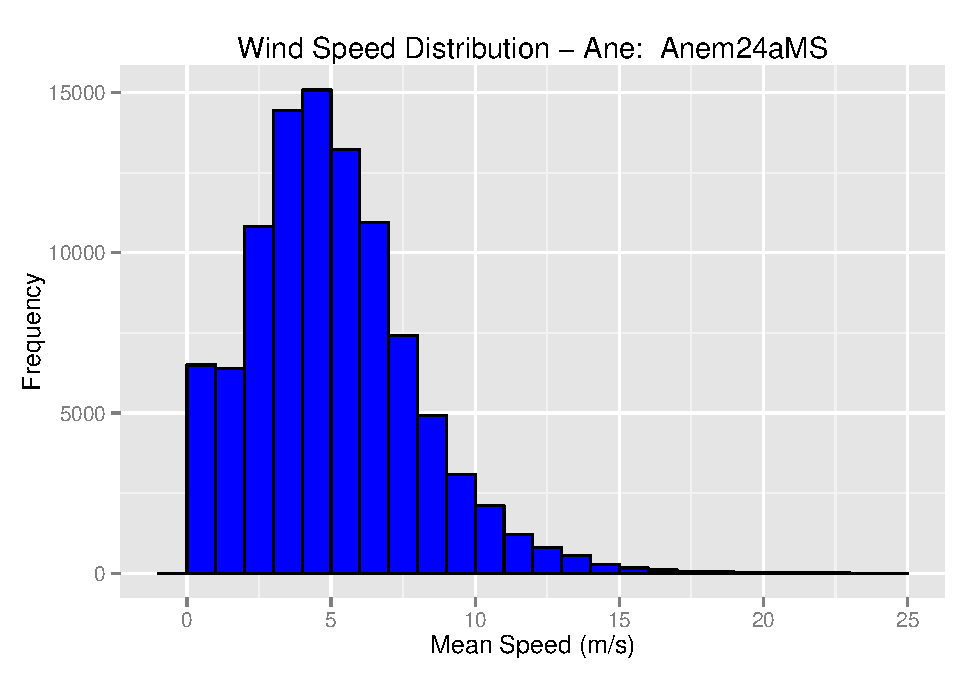
\includegraphics{Manual_WindResource_files/figure-latex/unnamed-chunk-9-1.pdf}
Gráfico 1. Histograma de velocidad de viento promedio para el anemómetro
``Anem24aMS''.

\begin{Shaded}
\begin{Highlighting}[]
\KeywordTok{plotWD} \NormalTok{(wdMtTom, }\DataTypeTok{ane=}\StringTok{"Anem24bMS"}\NormalTok{, }\DataTypeTok{var=}\StringTok{"ave"}\NormalTok{, }\DataTypeTok{type=}\StringTok{"histogram"}\NormalTok{, }\DataTypeTok{by=}\StringTok{"month"}\NormalTok{)}
\end{Highlighting}
\end{Shaded}

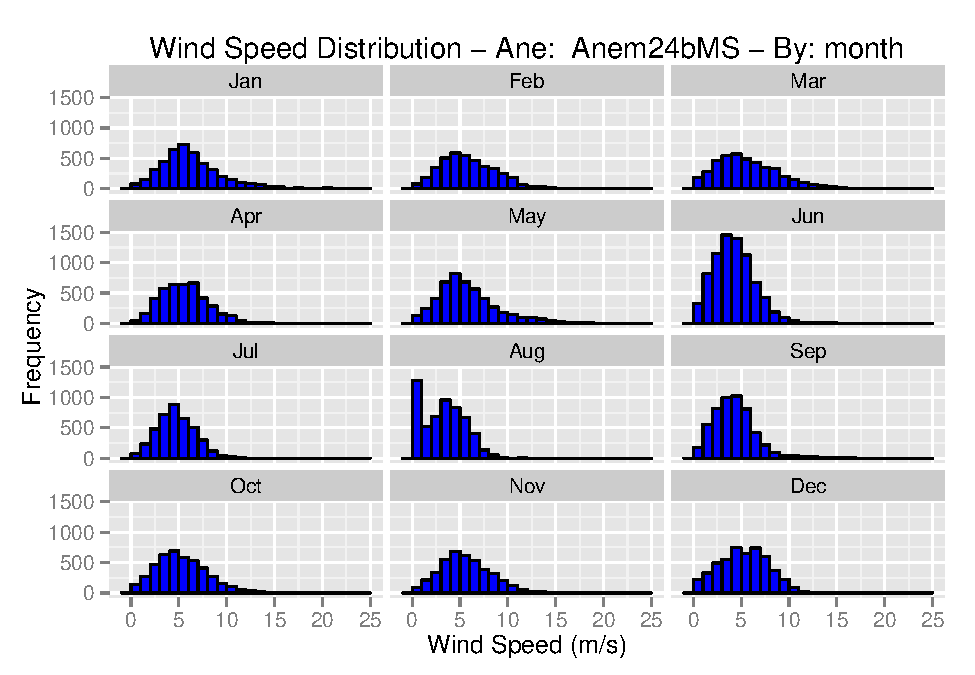
\includegraphics{Manual_WindResource_files/figure-latex/unnamed-chunk-10-1.pdf}
Gráfico 2. Histogramas mensuales de velocidad de viento promedio para el
anemómetro ``Anem24bMS''.

\begin{Shaded}
\begin{Highlighting}[]
\KeywordTok{plotWD} \NormalTok{(wdMtTom, }\DataTypeTok{ane=}\KeywordTok{c}\NormalTok{(}\StringTok{"Anem24aMS"}\NormalTok{,}\StringTok{"Anem37aMS"}\NormalTok{), }\DataTypeTok{var=}\StringTok{"mean"}\NormalTok{, }\DataTypeTok{type=}\StringTok{"rose"}\NormalTok{)}
\end{Highlighting}
\end{Shaded}

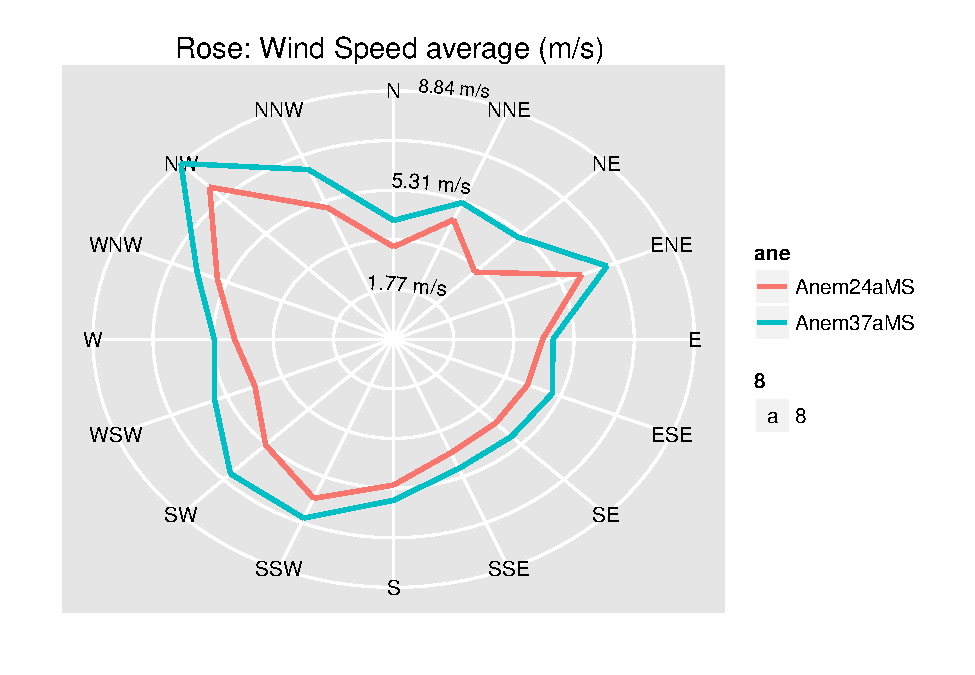
\includegraphics{Manual_WindResource_files/figure-latex/unnamed-chunk-11-1.pdf}
Gráfico 3. Rosas de viento de velocidad media para el anemómetros
``Anem24bMS'' y ``Anem24aMS''.

\begin{Shaded}
\begin{Highlighting}[]
\CommentTok{# plotWD (wdMtTom, ane="Anem24aMS", var="mean", type="rose", since='2000-02-01', to='2000-05-31', by='hour')}

\KeywordTok{plotWD} \NormalTok{(wdMtTom, }\DataTypeTok{ane=}\StringTok{"Anem24bMS"}\NormalTok{, }\DataTypeTok{var=}\StringTok{"mean"}\NormalTok{, }\DataTypeTok{type=}\StringTok{"rose"}\NormalTok{,  }\DataTypeTok{by=}\StringTok{'hour'}\NormalTok{)}
\end{Highlighting}
\end{Shaded}

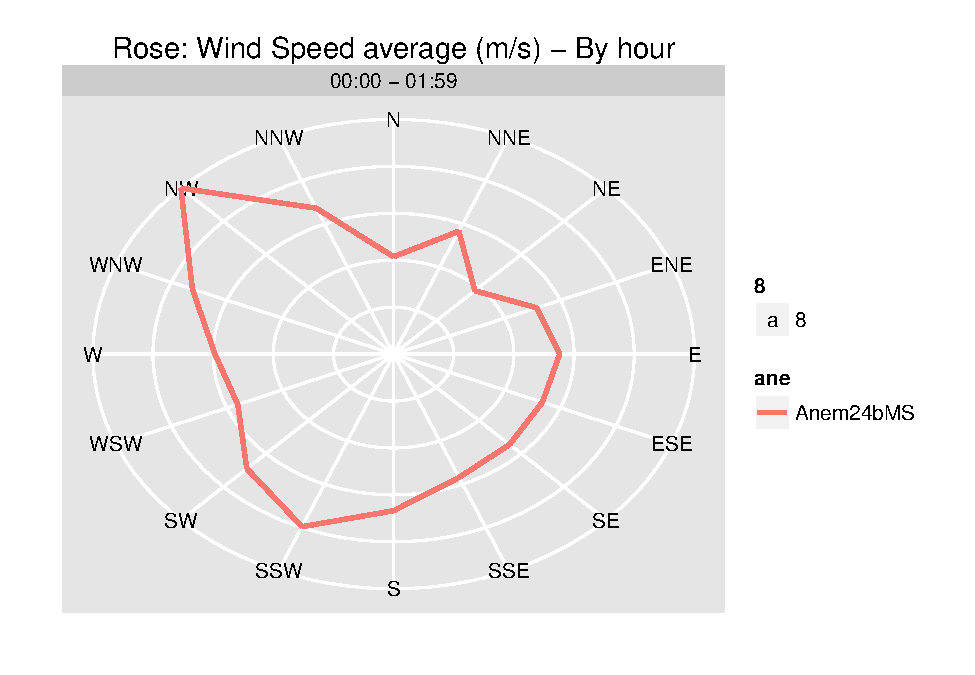
\includegraphics{Manual_WindResource_files/figure-latex/unnamed-chunk-12-1.pdf}
Gráfico 4. Rosas de viento de velocidad media para el anemómetro
``Anem24bMS'' a lo largo del día.

\begin{Shaded}
\begin{Highlighting}[]
\KeywordTok{plotWD} \NormalTok{(wdMtTom, }\DataTypeTok{ane=}\StringTok{"Anem24aMS"}\NormalTok{,  }\DataTypeTok{type=}\StringTok{"boxplot"}\NormalTok{, }\DataTypeTok{by=}\StringTok{'hour'}\NormalTok{)}
\end{Highlighting}
\end{Shaded}

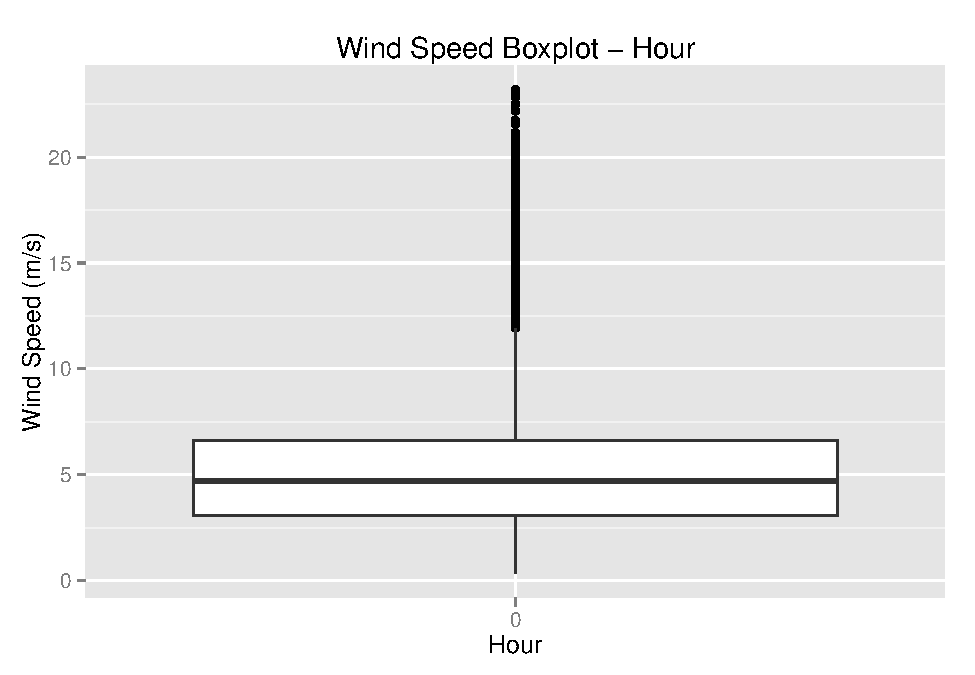
\includegraphics{Manual_WindResource_files/figure-latex/unnamed-chunk-13-1.pdf}
Gráfico 5. Gráfico Boxplot para las 24 horas del día.

\begin{Shaded}
\begin{Highlighting}[]
\CommentTok{#plotWD (wdMtTom, ane=c("Anem24aMS","Anem37aMS"), var="mean", type="profile", by='month')}
\end{Highlighting}
\end{Shaded}

Gráfico 5. Gráfico de perfiles a lo largo del mes.

\section{3.2 Tablas}\label{tablas}

El módulo tablas, permite obtener tablas de resumen de información que a
su vez pueden ser guardadas en una variable y exportadas en formato .csv
o similar. Por simplicidad, para la función \texttt{tableWD()}, utiliza
exactamente los mismos parámetros de la función \texttt{plotWD()}.\\A
modo de ejemplo, se muestran los resultados de dos funciones mostradas
anteriormente:

\begin{Shaded}
\begin{Highlighting}[]
\KeywordTok{tableWD} \NormalTok{(wdMtTom, }\DataTypeTok{ane=}\StringTok{"Anem24aMS"}\NormalTok{, }\DataTypeTok{var=}\StringTok{"mean"}\NormalTok{, }\DataTypeTok{type=}\StringTok{"histogram"}\NormalTok{)}
\end{Highlighting}
\end{Shaded}

\begin{verbatim}
##    Lower Upper  Freq
## 1      0     1  6553
## 2      1     2  6483
## 3      2     3 10809
## 4      3     4 14508
## 5      4     5 14914
## 6      5     6 13230
## 7      6     7 10938
## 8      7     8  7410
## 9      8     9  4999
## 10     9    10  3073
## 11    10    11  2045
## 12    11    12  1197
## 13    12    13   791
## 14    13    14   553
## 15    14    15   282
## 16    15    16   160
## 17    16    17    97
## 18    17    18    44
## 19    18    19    36
## 20    19    20    12
## 21    20    21    15
## 22    21    22     4
## 23    22    23     4
## 24    23    24     2
\end{verbatim}

Gráfico 4. Rosa de viento para las medias de los anemómetros
``Anem24aMS'' y ``Anem24bMS''.

\begin{Shaded}
\begin{Highlighting}[]
\KeywordTok{tableWD} \NormalTok{(wdMtTom, }\DataTypeTok{ane=}\StringTok{"Anem24bMS"}\NormalTok{, }\DataTypeTok{var=}\StringTok{"mean"}\NormalTok{, }\DataTypeTok{type=}\StringTok{"histogram"}\NormalTok{, }\DataTypeTok{by=}\StringTok{"month"}\NormalTok{)}
\end{Highlighting}
\end{Shaded}

\begin{verbatim}
##    Lower Upper Jan Feb Mar Apr May  Jun Jul  Aug  Sep Oct Nov Dec
## 1      0     1  81  79 195  53 132  330  74 1285  184 146  86 223
## 2      1     2 156 194 280 170 247  828 241  533  568 273 215 330
## 3      2     3 317 350 465 414 412 1147 482  683  808 468 341 495
## 4      3     4 451 507 544 582 686 1458 728  961  995 633 556 553
## 5      4     5 641 580 570 631 806 1385 864  825 1010 677 676 736
## 6      5     6 731 551 489 636 683 1125 653  664  810 584 621 650
## 7      6     7 595 470 434 665 566  669 508  405  417 528 539 738
## 8      7     8 422 362 349 419 412  423 299  135  216 410 385 595
## 9      8     9 320 342 333 290 277  195 118   52   94 280 318 378
## 10     9    10 196 243 206 160 174   92  47   11   51 162 206 221
## 11    10    11 147 175 142 117 138   50  18    1   40 102 117  85
## 12    11    12 109  71 109  42 100   17   7    3   28  60  58  25
## 13    12    13  91  40  66  19  92   13   0    0   20  36  29  12
## 14    13    14  74  30  46  11  74    6   0    0    9  25  16   5
## 15    14    15  39  15  28   7  43    8   0    0    2   6   7   0
## 16    15    16  28   6  21   5  25    1   0    0    2   6   4   1
## 17    16    17   7   7  10   3  15    3   1    0    4   2   4   0
## 18    17    18  15   0   4   0   8    1   0    0    0   2   0   0
## 19    18    19   9   0   2   2   6    0   0    0    0   0   0   0
## 20    19    20   5   0   0   0   4    0   0    0    0   0   0   0
## 21    20    21  12   0   0   0   0    0   0    0    0   0   0   0
## 22    21    22   5   0   0   0   0    0   0    0    0   0   0   0
## 23    22    23   4   0   0   0   0    0   0    0    0   0   0   0
## 24    23    24   3   0   0   0   0    0   0    0    0   0   0   0
\end{verbatim}

Tabla 4. Valores mínimos de la velocidad del viento por punto cardinal.

\begin{Shaded}
\begin{Highlighting}[]
\KeywordTok{tableWD} \NormalTok{(wdMtTom, }\DataTypeTok{ane=}\KeywordTok{c}\NormalTok{(}\StringTok{"Anem24aMS"}\NormalTok{,}\StringTok{"Anem37aMS"}\NormalTok{), }\DataTypeTok{var=}\StringTok{"mean"}\NormalTok{, }\DataTypeTok{type=}\StringTok{"rose"}\NormalTok{)}
\end{Highlighting}
\end{Shaded}

\begin{verbatim}
##    rose       ane ang.start value.start
## 1     N Anem24aMS      22.5    4.602575
## 2     N Anem37aMS      22.5    5.259513
## 3   NNE Anem24aMS      45.0    3.373706
## 4   NNE Anem37aMS      45.0    5.147688
## 5    NE Anem24aMS      67.5    5.983362
## 6    NE Anem37aMS      67.5    6.788557
## 7   ENE Anem24aMS      90.0    4.380959
## 8   ENE Anem37aMS      90.0    4.686879
## 9     E Anem24aMS     112.5    4.263812
## 10    E Anem37aMS     112.5    5.051579
## 11  ESE Anem24aMS     135.0    4.237781
## 12  ESE Anem37aMS     135.0    4.905252
## 13   SE Anem24aMS     157.5    4.385813
## 14   SE Anem37aMS     157.5    4.994153
## 15  SSE Anem24aMS     180.0    5.196715
## 16  SSE Anem37aMS     180.0    5.737979
## 17    S Anem24aMS     202.5    6.137197
## 18    S Anem37aMS     202.5    6.900500
## 19  SSW Anem24aMS     225.0    5.323107
## 20  SSW Anem37aMS     225.0    6.784383
## 21   SW Anem24aMS     247.5    4.410994
## 22   SW Anem37aMS     247.5    5.691546
## 23  WSW Anem24aMS     270.0    4.675592
## 24  WSW Anem37aMS     270.0    5.274543
## 25    W Anem24aMS     292.5    5.610432
## 26    W Anem37aMS     292.5    6.255026
## 27  WNW Anem24aMS     315.0    7.653249
## 28  WNW Anem37aMS     315.0    8.844021
## 29   NW Anem24aMS     337.5    5.062725
## 30   NW Anem37aMS     337.5    6.535627
## 31  NNW Anem24aMS     360.0    3.283790
## 32  NNW Anem37aMS     360.0    4.227266
\end{verbatim}

Tabla 5. Frecuencias obtenidas por punto cardinal.

\begin{Shaded}
\begin{Highlighting}[]
\CommentTok{# tableWD (wdMtTom, ane="Anem24aMS", var="mean", type="rose", since='2000-02-01', to='2000-05-31', by='hour')}

\KeywordTok{tableWD} \NormalTok{(wdMtTom, }\DataTypeTok{ane=}\StringTok{"Anem24bMS"}\NormalTok{, }\DataTypeTok{var=}\StringTok{"mean"}\NormalTok{, }\DataTypeTok{type=}\StringTok{"rose"}\NormalTok{,  }\DataTypeTok{by=}\StringTok{'hour'}\NormalTok{)}
\end{Highlighting}
\end{Shaded}

\begin{verbatim}
##    rose       ane ang.start          hour value.start
## 1     N Anem24bMS      22.5 00:00 - 01:59    4.369238
## 2   NNE Anem24bMS      45.0 00:00 - 01:59    2.945470
## 3    NE Anem24bMS      67.5 00:00 - 01:59    3.972085
## 4   ENE Anem24bMS      90.0 00:00 - 01:59    4.258324
## 5     E Anem24bMS     112.5 00:00 - 01:59    4.129467
## 6   ESE Anem24bMS     135.0 00:00 - 01:59    4.205217
## 7    SE Anem24bMS     157.5 00:00 - 01:59    4.388078
## 8   SSE Anem24bMS     180.0 00:00 - 01:59    5.147953
## 9     S Anem24bMS     202.5 00:00 - 01:59    6.140311
## 10  SSW Anem24bMS     225.0 00:00 - 01:59    5.324648
## 11   SW Anem24bMS     247.5 00:00 - 01:59    4.326644
## 12  WSW Anem24bMS     270.0 00:00 - 01:59    4.581549
## 13    W Anem24bMS     292.5 00:00 - 01:59    5.586499
## 14  WNW Anem24bMS     315.0 00:00 - 01:59    7.714175
## 15   NW Anem24bMS     337.5 00:00 - 01:59    5.190672
## 16  NNW Anem24bMS     360.0 00:00 - 01:59    3.200493
\end{verbatim}

Tabla 5. Frecuencias obtenidas por punto cardinal.

\begin{Shaded}
\begin{Highlighting}[]
\CommentTok{#tableWD (wdMtTom, ane=c("Anem24aMS","Anem37aMS"), var="mean", type="profile", by='month')}
\end{Highlighting}
\end{Shaded}

\subsection{3.3 Otros gráficos}\label{otros-graficos}

El paquete incluye dos funciones adicionales mas, que utilizan las
funciones de google a ravés de GoogleViz. Dado que los parámetros de
estas gráficos no coinciden con los anteriores, tienen dos funciones
específicas: \texttt{plotwindserie()} y \texttt{plotcalendar()}.

El primero de ellos es un gráfico interactivo de las series de valores,
que permiten recorrer las series de datos (velocidad media, minimos,
máximos, desvíos, presión y temperatura). Utiliza unos componentes
desarrollados por Google que permiten realizar zooms y recorrer
interactivamente las series de datos.

\begin{Shaded}
\begin{Highlighting}[]
\KeywordTok{plotwindserie}\NormalTok{(wdMtTom, }\DataTypeTok{year=}\DecValTok{2000}\NormalTok{, }\DataTypeTok{month=}\DecValTok{01}\NormalTok{, }\DataTypeTok{var=}\KeywordTok{c}\NormalTok{(}\StringTok{"mean"}\NormalTok{))}
\end{Highlighting}
\end{Shaded}

\begin{verbatim}
## starting httpd help server ... done
\end{verbatim}

El segundo gráfico, conocido como \texttt{calendar}, permite apreciar de
forma simple los valores promedios de velocidad para los distintos dias
y además es una poderosa herramienta para determinar datos faltantes.

\begin{Shaded}
\begin{Highlighting}[]
\CommentTok{# plotcalendar(wdMtTom, var="mean", ane="Anem37aMS", shiny=F)}
\end{Highlighting}
\end{Shaded}

\section{4 Ajuste de distribuciones}\label{ajuste-de-distribuciones}

Uno de los análisis mas frecuente a la hora de estudiar series de
vientos para su uso eólico, es el estudio de su distribución de
probabilidad. Si bien en la gran mayoría de los casos la distribución
utilizada es la distribución de Weibull, también existen antecedentes de
casos en los cuales en el mejor ajuste se logró con otras dictribuciones
de asimetría positiva, como la distribución de Gamma o incluso la
LogNormal.

El ajuste de los datos a estas tres distribuciones de probabilidad puede
realizarse utilizando las funciones \texttt{plotWD()} y
\texttt{tableWD()} indicando \texttt{"fit"} en el parámetro type.

\begin{Shaded}
\begin{Highlighting}[]
\KeywordTok{plotWD} \NormalTok{(wdMtTom, }\DataTypeTok{ane=}\StringTok{"Anem24aMS"}\NormalTok{, }\DataTypeTok{type=}\StringTok{"fit"}\NormalTok{)}
\end{Highlighting}
\end{Shaded}

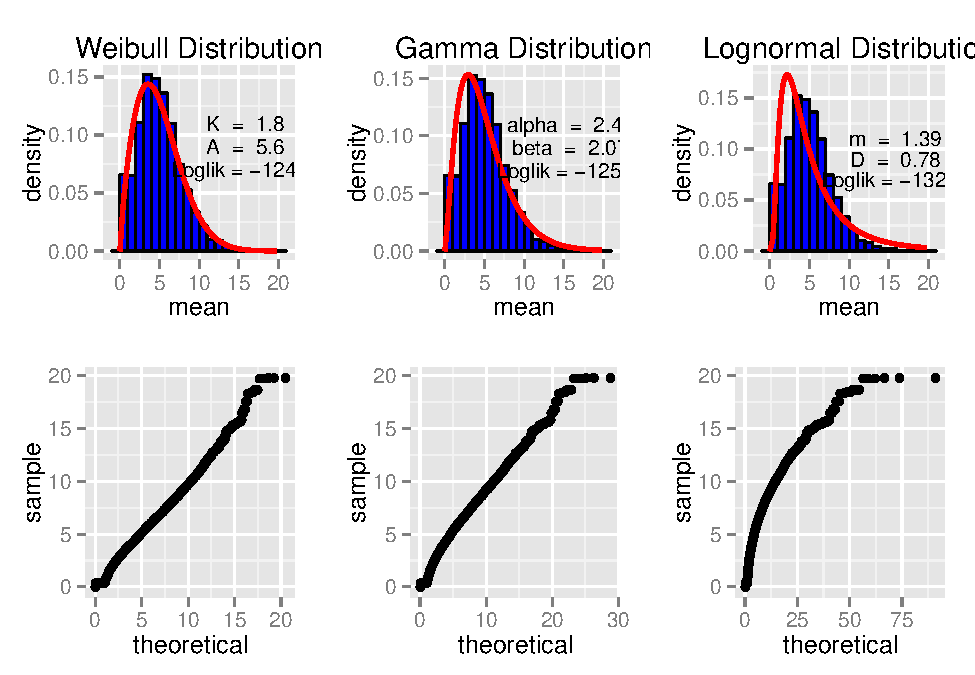
\includegraphics{Manual_WindResource_files/figure-latex/unnamed-chunk-22-1.pdf}
Gráfico 8. Comparación de los ajustes de distribución

Es posible apreciar los histogramas empíricos y junto con la curva
teórica ajustada y los respectivos QQplot que permiten evaluar la bondad
e ajuste de los mismos. Para obtener los valores de parametros estimados
junto con la verosimilitud y los Akaike, utilizamos la función
\texttt{tableWD()} de la siguiente manera:

\begin{Shaded}
\begin{Highlighting}[]
\KeywordTok{tableWD} \NormalTok{(wdMtTom, }\DataTypeTok{ane=}\StringTok{"Anem24aMS"}\NormalTok{, }\DataTypeTok{type=}\StringTok{"fit"}\NormalTok{)}
\end{Highlighting}
\end{Shaded}

\begin{verbatim}
##              Parameter1   Parameter2 loglik   aic
## Weibull       k= 1.8005    C= 5.5974 -12403 24809
## Gamma     alpha= 2.4198 beta= 2.0666 -12576 25154
## Lognormal      m= 1.389    D= 0.7813 -13231 26465
\end{verbatim}

wd10\$ane{[}{[}``nane''{]}{]} \textless{}- 2
wd10{[}{[}``interval.minutes''{]}{]} \textless{}- 10 turbulence(wd10,
ane=``ane10'') plotWD (wd10, ane=``ane10'', type=``turbulence'')

\section{5 Análisis de turbulencia}\label{analisis-de-turbulencia}

Otra análisis de interés Para especificar el tipo de gráfico se utiliza
el parámetro type, pudiendo optar entre histogramas, rosas de viento,
boxplot, y series temporales. Para este último caso, se integró el
paquete GoogleVis que brinda una intuitiva interfaz web para
visualización de series (ver Gráfico 2).\\Un tercer parámetro ane,
permite indicar de qué anemómetro/s se desean considerar en los
gráficos.

\begin{Shaded}
\begin{Highlighting}[]
\KeywordTok{data}\NormalTok{(wd10)}
\KeywordTok{plotWD} \NormalTok{(}\DataTypeTok{data=}\NormalTok{wd10, }\DataTypeTok{type=}\StringTok{"turbulence"}\NormalTok{,}\DataTypeTok{ane=}\KeywordTok{c}\NormalTok{(}\StringTok{"ane10"}\NormalTok{))}
\end{Highlighting}
\end{Shaded}

\begin{figure}[htbp]
\centering
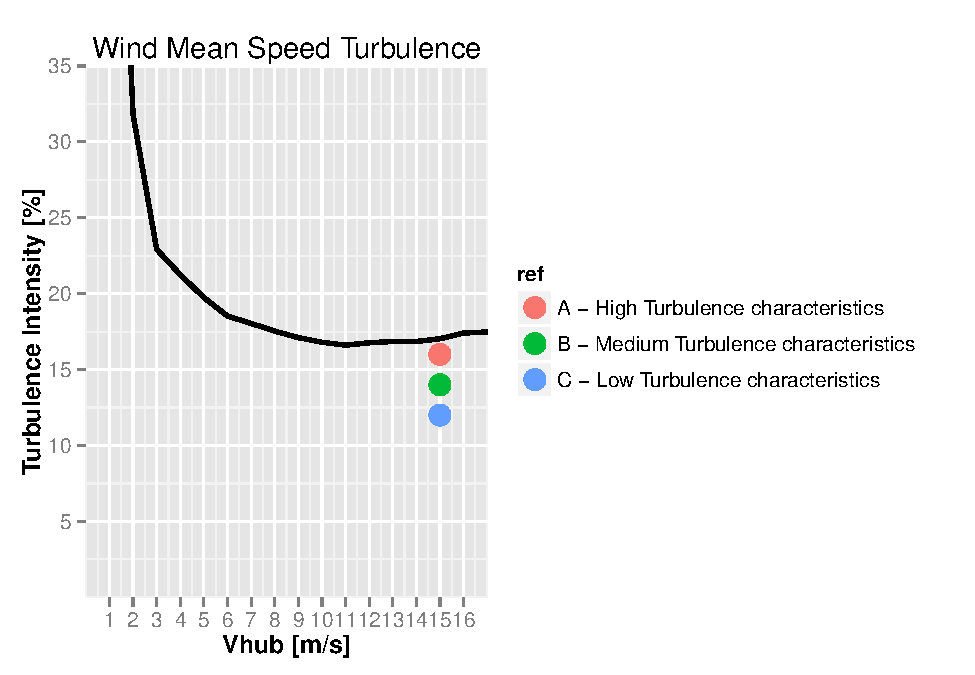
\includegraphics{Manual_WindResource_files/figure-latex/unnamed-chunk-24-1.pdf}
\caption{}
\end{figure}

\section{5. Interfaz web}\label{interfaz-web}

Una de las principales dificultades con las que se encuentran los
usuarios de R, es una curva de aprendizaje lenta y
pronunciada.\\Teniendo en cuenta que los potenciales usuarios de la
aplicación pueden tener poca experiencia en R, se ha desarrollado una
interfaz web utilizando el paquete R \texttt{shiny}. La misma permite
operar el sistema desde una interfaz web amigable para el usuario no
familiarizado con R. En el gráfico 3, se muestra una captura de esta
interfaz a modo de ejemplo.

\begin{Shaded}
\begin{Highlighting}[]
\KeywordTok{runGUI}\NormalTok{(wdMtTom)}
\end{Highlighting}
\end{Shaded}

\begin{verbatim}
## NULL
\end{verbatim}

También es posible acceder a una versión online:
\url{https://mbonoli.shinyapps.io/WindResource}

\section{6. Conclusiones}\label{conclusiones}

El paquete WindResource para R brinda herramientas para la
caracterización de recuso eólico similar a la que ofrecen los softs
comerciales.\\Para validar las salidas del paquete, el INTI Neuquén
colabora suministrando los datos de recurso eólico de su centro de
evaluación de aerogeneradores de baja potencia sito en la ciudad de
Cutral Có, provincia del Neuquén. En contra partida este trabajo
entrega, a tal institución, sus resultados.

\end{document}
